%--------------------------------------------------------------------
%
%Mustervorlage fuer eine Aufgabe
%
%--------------------------------------------------------------------
%
%Ueberschreiben der automatisch erzeugten Aufgabennummer
%Die folgende Aufgabennummer ergibt sich aus dem Stand des
%Z�hlers + 1
%\setcounter{chapter}{0}
%
%
% 10 pages
\chapter{Theoretical Background}\label{chap:literatureReview}
%
The core of the field of mechatronics is the combination of both hardware and software. A fundamental aspect in the field of mechatronics is the modularisation. Modularisation takes place both on the hardware and on the software level. The hardware modules used in this project are a differential driver robot and a triangulation laser scanner. On the other side, ROS is responsible for the implementation of the software modules.  
Before going deep into the implementation of the project and the methods used to solve the problem,  both software and hardware modules will be explained.
%
%Teilaufgabe 1
%
\section{Robots Operating System ROS}\label{sec:ros}
%3 pages
Designing robots in general, especially mobile robots, is considered as one of the essential elements of the industrial revolutions over the past decades.  However, designing a robot is a complicated procedure. The main reason for that complicity is that robots' platforms consist of two main components, namely the hardware and the software applications. 

The hardware of robots could be, i.e., sensors, motors, and actuators. On the other hand, software applications are responsible for doing a specific functionality, such as navigation, localization, or object recognition \cite{calis_roboter_2020}.


\subsection{Robot Software Platforms}
In order to simplify the robots' design procedure, scientists and researches were trying to develop so-called "Robot Software Platforms."  In the literature, there seems to be no specific definition of Robot Software Platforms. However, robots software platforms can be interpreted as a middleware between the hardware components and the software modules, allowing developers to design seperated software modules, that could run on different hardware components without reprogramming the developed software module according to the different low-level drivers of each component \cite{joseph_learning_2018}\cite{yoonseok_ros_2017} \cite{calis_roboter_2020}. For example, a software module could be developed for navigation. By integrating this module in a robot software platform, it can run on different robots without dealing with each robot's underlying complexity. Using a proper robot software platform depends on each robot's purpose and requirements, as each platform has its advantages and disadvantages. One of the most used robot software platforms is ROS. ROS stands for Robot Operating System, which is confusing, since ROS is not an operating system by itself. Instead, it runs on an operating system like Linux and can be seen as a layer between an operating system and robot's applications, as shown in figure \ref{fig2_1} \cite{yoonseok_ros_2017}.
\begin{figure}[ht]
	\centering
	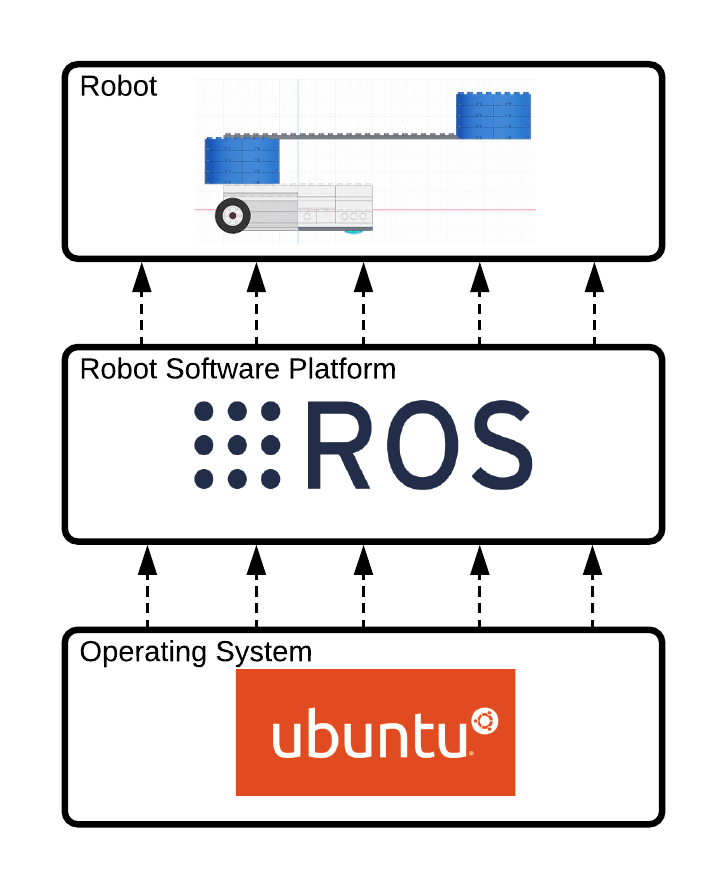
\includegraphics[width = 0.6 \textwidth, frame]{./Bilder/roslayers.png}			\caption{ROS as middleware between robots and operating systems}
	\label{fig2_1}
\end{figure}

ROS has been chosen over other platforms for the implementation of the application developed in this thesis because of its ecosystem and the enormous amount of packages that are ready to be used and integrated into the application. Another advantage of ROS is its simplicity to learn. One of the ROS disadvantages is that it is not a real-time robot software platform, as it is built on Linux. However, realtime applications can be developed on ROS2, which is the next version of ROS.
ROS versions are always tied to Ubuntu LTS (Long Term Support) versions and are released simultaneously, namely every two years. The used version of ROS in this project is ROS Melodic, which runs on Ubuntu 18.04. The next version of ROS is ROS Neotic, which runs on Ubuntu 20.04. ROS Noetic would be the last version of ROS. After that, ROS2 will be used instead.  


\subsection{ROS Working Principle}
ROS working principle is explained in the literature in different ways. As explained in \cite{calis_roboter_2020}, ROS is based on a publish/subscribe concept, where processes communicate with each other via a message system. The best way to explain how ROS works is to analyze this publish/subscribe concept and explain the message system's main components and how messages are exchanged. This subsection explains the working principle of the ROS based on its description given in \cite{yoonseok_ros_2017}.

ROS applications consist of different processes, where each process is responsible for specific functionality such as navigation, path planning, or processing sensor data and so forth. These processes are called nodes. These nodes exchange information with each other in the form of messages. Each node can contain a publisher, that sends messages to a topic, or a subscriber, that receives messages from a topic, or both. A topic can be interpreted as a container that contains messages in nodes. TCPROS is the protocol that is responsible for exchanging the messages between different nodes in ROS, and it is based on a TCP/IP protocol. 
The central node in any ROS application is the master node, which is responsible for matching the information of the nodes with each other. In figure \ref{fig2_2}, the steps needed for establishing a communication between a publisher node and a subscriber node is displayed. First, the subscriber sends its information to the master node. This information contains, for example, the URI of the node, and the topics in the node. Next, the publisher sends its information to the master. The master then passes the publisher's information to the subscriber. The subscriber now recognizes the publisher, and the communication is established. The task of the master node is only to exchange the nodes' information. Once the nodes recognize each other, the master node role is completed.
ROS nodes also contain other information other than publishers and subscribers, such as parameters, service servers, and action servers. 
\begin{figure}[ht]
	\centering
	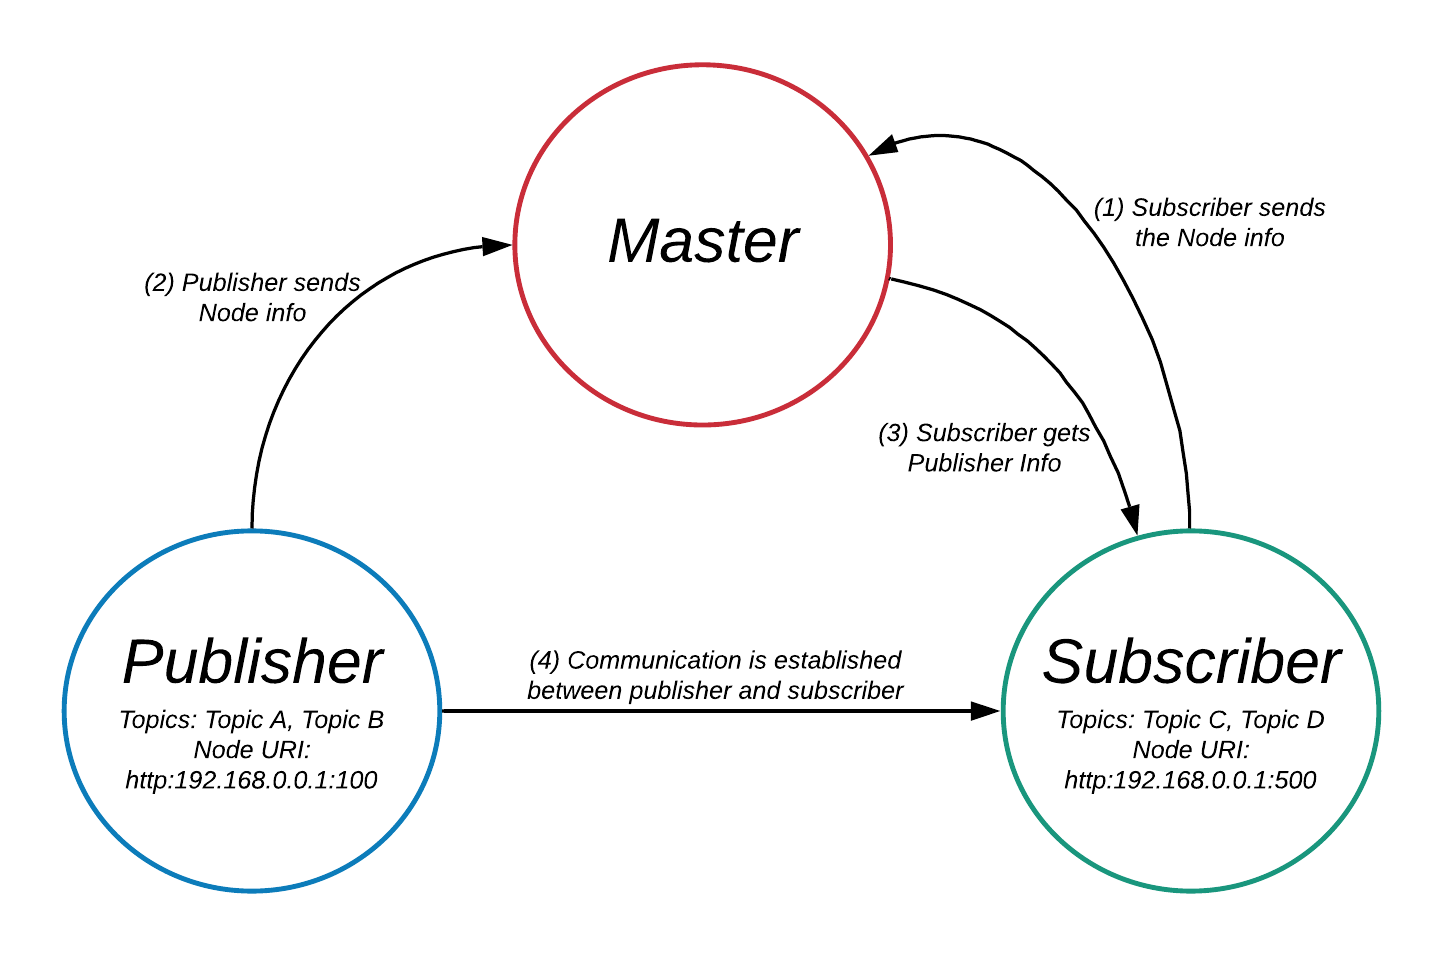
\includegraphics[width = 0.8\textwidth, frame]{./Bilder/umlROS.png}			\caption{ROS architecture design}
	\label{fig2_2}
\end{figure}


As described in \cite{noauthor_catkin_nodate}, ROS has its own build system, which is called catkin. In each ROS project, a file called "CMakeLists.txt" must be defined. This file contains the dependencies of the project that are needed for the build process. Catkin is also responsible for creating the workspace, in which all project components are installed. Inside the catkin workspace, the project packages are defined. Packages in ROS can be interpreted as libraries. Each package contains files, in which nodes, messages, services, and functionalities are defined.


In summary, it is important to know that ROS's core feature is the modularization in terms of software. Modularization has many advantages, such as code reuse and working on loosely coupled processes.  
%
%--------------------------------------------------------------------
%
%
\section{Differential Driver Robots}\label{sec:legoboost}
%3 pages

The definition of mobile robots is usually associated with autonomous movement. As explained in \cite{tzafestas_introduction_2013}, mobile robots are autonomously moving robots that can reach a specific goal. Therefore, an essential property of mobile robots is that they can plan their motion independently. Mobile robots are differentiated based on the environment they are used in, such as air, ground, and water \cite{rubio_review_2019}. Thus, the definition of mobile robots does not just include wheeled mobile robots, but generally, any robot that can move autonomously, such as drones, wheeled robots, or even legged robots. As shown in figure \ref{fig2_3}, wheeled mobile robots can be classified into three main categories: car-like mobile robots, omnidirectional mobile robots, and differential mobile robots \cite{tzafestas_introduction_2013}. 

\begin{figure}[ht]
\centering
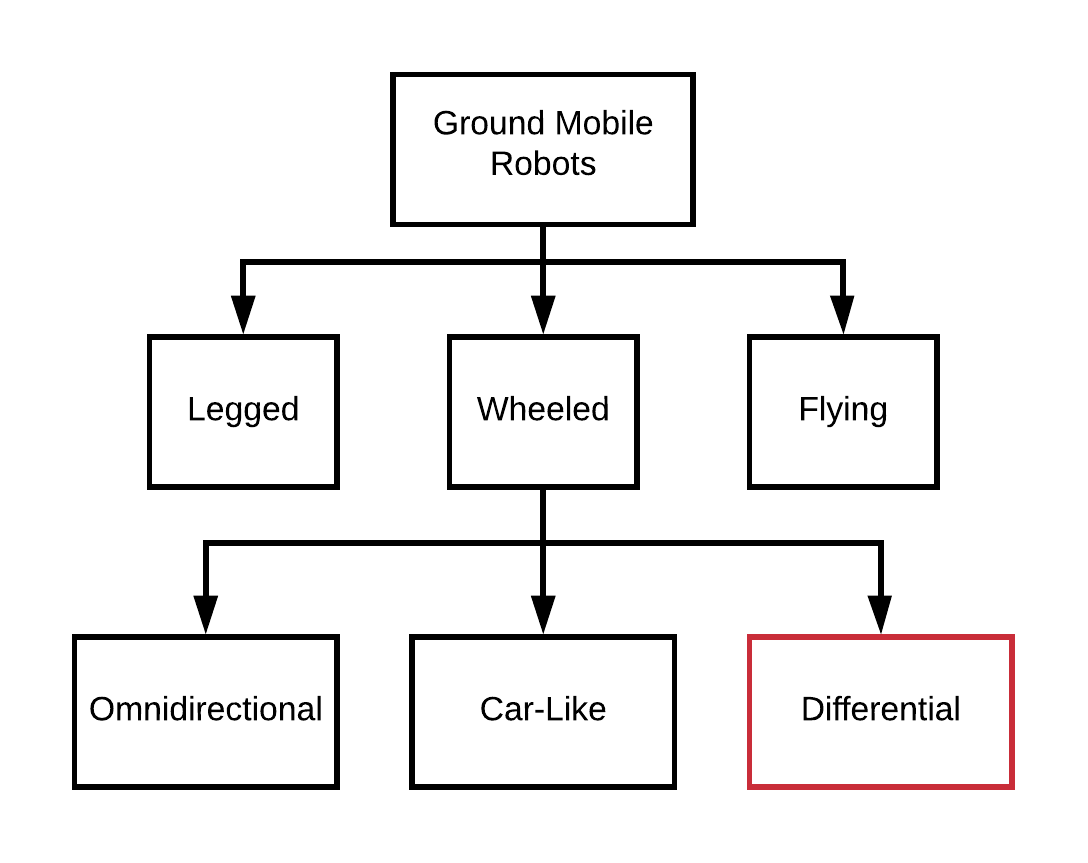
\includegraphics[width = 0.6\textwidth, frame]{./Bilder/robottypes.png}
\caption{Different types of ground mobile robots}
\label{fig2_3}
\end{figure}

The difference between these categories relies on the driving system of each robot. This subsection gives a theoretical explanation of the differential mobile robots since it is the type of mobile robot used for the project.

Differentially driven mobile robots are used in various applications, such as internal logistics or automated gastronomy, due to its design simplicity. As shown in figure \ref{fig2_4}, the drive system of differentially driven mobile robots consists of two wheels placed on the right and the left side of the robot, where each wheel is controlled by a separate motor \cite{tzafestas_introduction_2013}. Moreover, most of the time, there is one more omnidirectional wheel or a caster wheel that provides the stability of the robot enables the robot to move even on uneven surfaces. The speed and direction of the right and left wheels determine the robot's motion. By using different wheel speeds and directions, the motion of differentially driven robots can be explained as an arc around a point, which is the Instantaneous Center of Rotation (ICR), as shown in figure \ref{fig2_4} \cite{corke_robotics_2017}. 
\begin{figure}[ht]
\centering
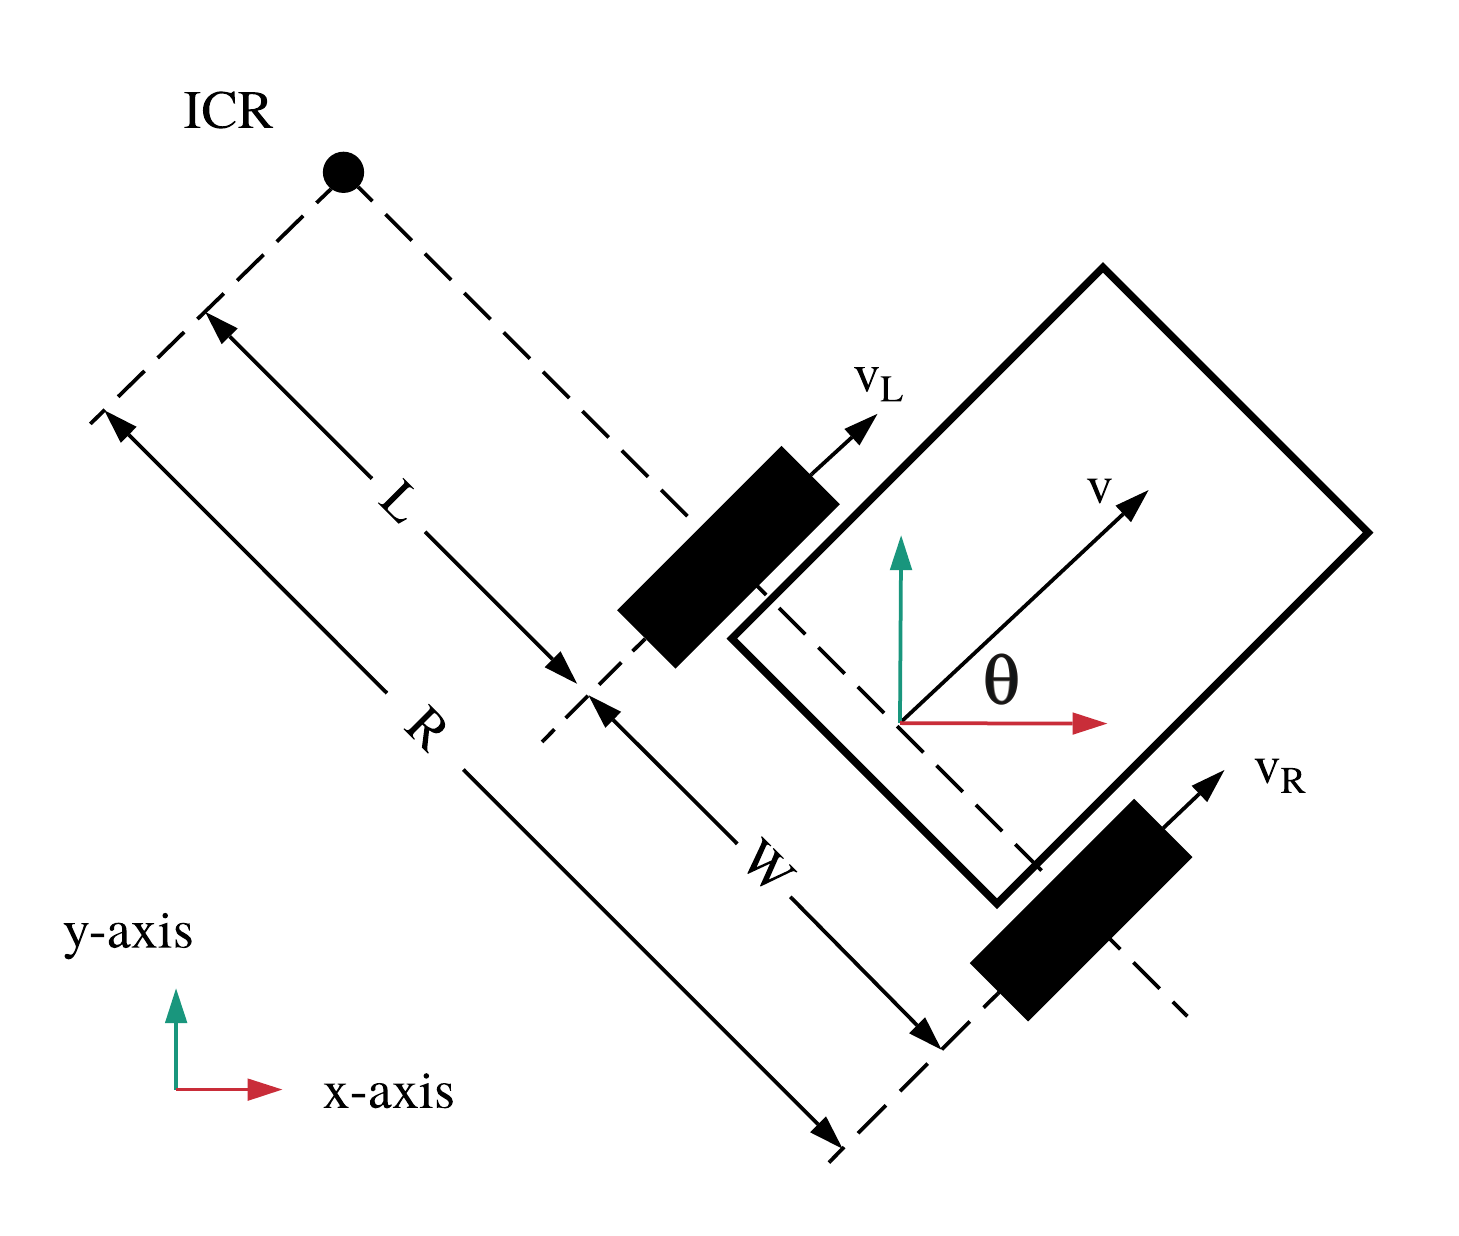
\includegraphics[width = 0.7\textwidth, frame]{./Bilder/differentialdrive.png}
\caption{Basic design of a differential driven mobile robot}
\label{fig2_4}
\end{figure}
The properties of the ICR, namely, the distance between the robot and the ICR, can be determined by knowing the velocity of each wheel and the distance between the wheels. This kinematic model is explained in \cite{corke_robotics_2017} as follows:

\begin{equation} \label{eq2_1}
\dot{\theta} = \frac{v_L}{L} = \frac{v_R}{R} 
\end{equation}
\begin{equation} \label{eq2_2}
\dot{\theta} = \frac{v_R-v_L}{W} 
\end{equation}
\begin{equation} \label{eq2_3}
\dot{x} = v \cdot cos(\theta)\\
\end{equation}
\begin{equation} \label{eq2_4}
\dot{y} = v \cdot sin(\theta)\\
\end{equation}
\begin{equation} \label{eq2_5}
\dot{\theta} =\frac{v_\Delta}{W}
\end{equation}
where \hspace{13mm} $v_L, v_R$ are the velocities of left and right wheels, respectively\\ 
	  \hspace*{25mm} $L, R$ are the distance from IPC to the left and right wheels, respectively\\
 	  \hspace*{25mm} $W$ is the distance between the left and right wheels\\
 	  \hspace*{25mm} $v_\Delta$ = $v_R-v_L$\\
 	  \hspace*{25mm} $v$ = $\frac{1}{2}\cdot(v_R+v_L)$\\
	  

By using these equations, a controller can be designed to achieve a specific goal such as, following a trajectory, or following a line, or moving to a specific point. The implementation of controllers is explained in a later chapter.
%
%
%--------------------------------------------------------------------
%
%

\section{Triangulation Laser Scanner}\label{sec:lidar}
%1 pages

Another module of the project is the laser scanner. The laser scanner is used to localize the differential driver robot position and orientation. The implementation of the localization process is discussed in later chapters. In this section, the advantage of the triangulation laser scanner compared to other types of sensors is discussed as well as the working principle of the specific sensor used.

\subsection{Localization Sensors and Methods}
\textbf{Wheel Odometry:}\\
The position of the robot can be estimated by using  rotary encoders. The rotary encoders are embedded in each wheel. The idea behind odometry sensors is to calculate the number of revolutions of the wheel.  By knowing the radius of the wheel, the moved distance can be then calculated. The wheel odometry method is simple and is used in many applications. However, several problems occur while implementing this method. As described in \cite{aqel_review_2016}, the main problem is the position draft due to the wheel slippage. This leads to inaccurate position estimation.

\textbf{GPS:}\\
Global Positioning System (GPS) is another localization method that can be used. It is used in different applications as transportations, agriculture, and aviation. Using a GPS receiver, the position of the robot can be determined with the help of four satellites. The main problem with using a GPS sensor is its measurement accuracy. For example, Adafruit Ultimate GPS has an accuracy of 3 meters and costs around 40\euro  \cite{industries_adafruit_nodate}. Another sensor is SparkFun GPS-RTK2, which has an accuracy of 2.5 meters and costs around 200 \euro \cite{noauthor_sparkfun_nodate}. Another problem is the reduction of accuracy in indoor applications. Thus, GPS sensor-based applications are used outdoors due to week signals from the GPS satellites.

\textbf{Ultrasonic Sensors:}\\
Ultrasonic sensors measure the distance to an obstacle by using ultrasonic waves. As described in \cite{aqel_review_2016}, the major disadvantage of ultrasonic sensors is the dependence on the material and the orientation of the measured object surface. Another disadvantage of the ultrasonic sensors is the poor lateral resolution (also called angular resolution) Additionally, the noise of the environment affects the accuracy of the measurement. In figure \ref{ultrasonic} is an example of ultrasonic sensors.

\begin{figure}[ht]
\centering
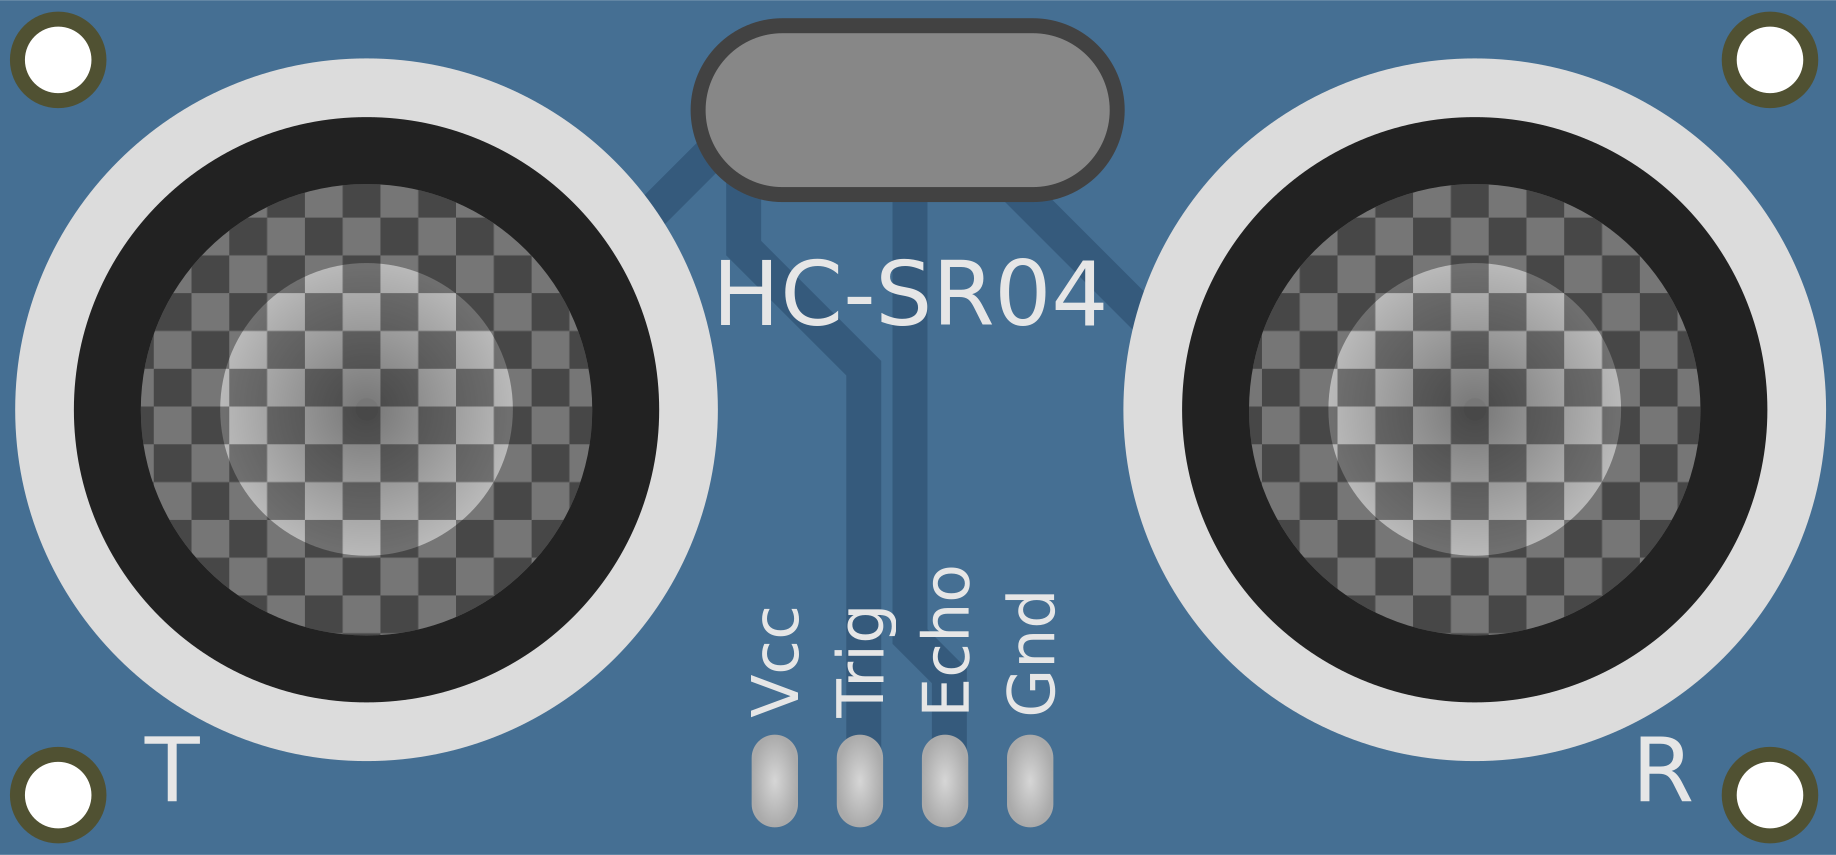
\includegraphics[width = 0.5\textwidth, frame]{./Bilder/Ultrasonic.png}
\caption{Ultrasonic sensor}
\label{ultrasonic}
\end{figure}

\textbf{Laser Sensors:}\\
Laser sensors are widely used for navigation and localization purposes. The application purpose of laser sensors is similar to ultrasonic sensors, where the distances to objects are detected. Laser sensors, however, as the name indicates, use a laser instead of ultrasonic waves. Laser sensors can be specified into two main types, namely position-based (triangulation) or time-based (LIDAR) sensors. LIDAR sensors calculate the distance to an object by measuring the time the laser took from the laser source to the object and back.  An example of LIDAR sensors is the Sick 2D-Laserscanner LMS100, which costs around 3000 \euro.

Triangulation Laser scanners use another technique to measure the distance to objects. It doesn't use the time of flight but the direction of the reflected light to determine the range of an object. In this project, the triangulation laser scanner YDLIDAR X2 which is displayed in figure \ref{ydlidar}, is used. It costs around 70 \euro, which is much cheaper than LIDAR sensors. The working principle of the triangulation laser scanner will be discussed in the following subsection. 

\begin{figure}[ht]
\centering
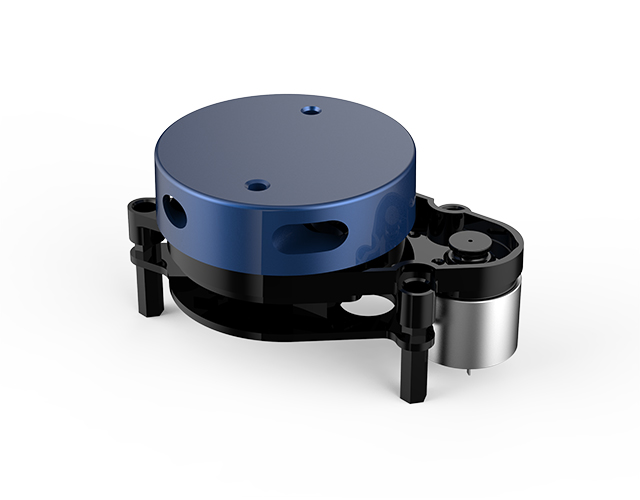
\includegraphics[width = 0.5\textwidth, frame]{./Bilder/ydlidar.jpg}
\caption{YDLIDAR X2 triangulation laser scanner. \textcopyright YDLIDAR All rights reserved }
\label{ydlidar}
\end{figure}

As explained in \cite{aqel_review_2016}, the following table describes the advantages and disadvantages of each method. 

\begin{table}[h]
\centering
\begin{tabular}{|| c | l | l ||} 
 \hline
 Sensor  & Advantages & Disadvantage \\ [0.5ex] 
 \hline\hline
 Wheel Odometry & \makecell[l]{Simple implementation \\ Cost-effective} & Position drift inaccuracy \\ 
 \hline
 GPS & Good for outdoor applications & \makecell[l]{ Low accuracy \\ Expensive} \\
 \hline
 Ultrasonic& \makecell[l]{Cost-effective} & \makecell[l]{Low accuracy due to poor lateral \\ resolution} \\
 \hline
 Laser sensor & \makecell[l]{Cost-effective \\ Good accuracy level} & \makecell[l]{Accuracy depends on reflection\\ properties of the surface\\} \\
 [1ex] 
 \hline
\end{tabular}
\caption{Comparison between different types of sensors}
\label{table:0}
\end{table}


\subsection{Triangulation Laser Scanner Working Principle}

The triangulation laser scanner consists of three main components, namely a laser, an optical lens, and and a position sensitive photo diode (PSD) also called "line detector" since the photodiodes form a line. When the laser hits an object, it reflects and travels to the line detector throw an optical lens, as displayed in figure \ref{triang}. 

\begin{figure}[ht]
\centering
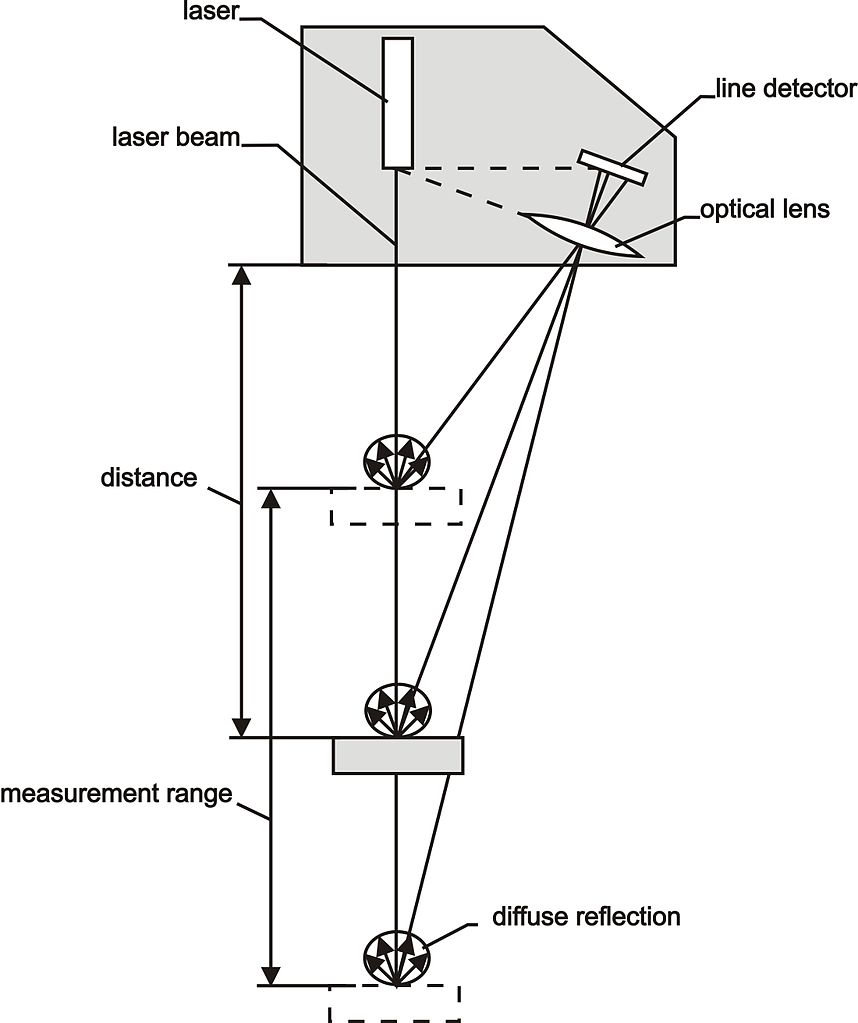
\includegraphics[width = 0.7\textwidth, frame]{./Bilder/triang.jpg}
\caption{Triangulation principle \cite{kwillms_english_2012}.}
\label{triang}
\end{figure}

The distance to this object is then calculated using the line detector. That is why it is called a position-based sensor.
The YDLIDAR X2 triangulation laser scanner rotates around its axis and scans the surrounding area with a scan angle of 360�. The angle resolution is 0.72�. The angle resolution is the angle difference between two consecutive scans.  These specifications are essential for the localization process and will be discussed in later chapters. In appendix \ref{chap:app1} the datasheet of the YDLIDAR X2 triangulation sensor is appended.


%
%
%--------------------------------------------------------------------
%
%
%
%
%--------------------------------------------------------------------
%
%
%
%
%--------------------------------------------------------------------
%
%